%% LyX 2.2.2 created this file.  For more info, see http://www.lyx.org/.
%% Do not edit unless you really know what you are doing.
\documentclass[english]{article}
\usepackage[T1]{fontenc}
\usepackage[latin9]{inputenc}
\usepackage{graphicx}
\usepackage{babel}
\usepackage{biolinum}

\begin{document}

\title{Plots}
\maketitle

\section{Data map}

\begin{minipage}{0.5\linewidth}
\begin{figure}
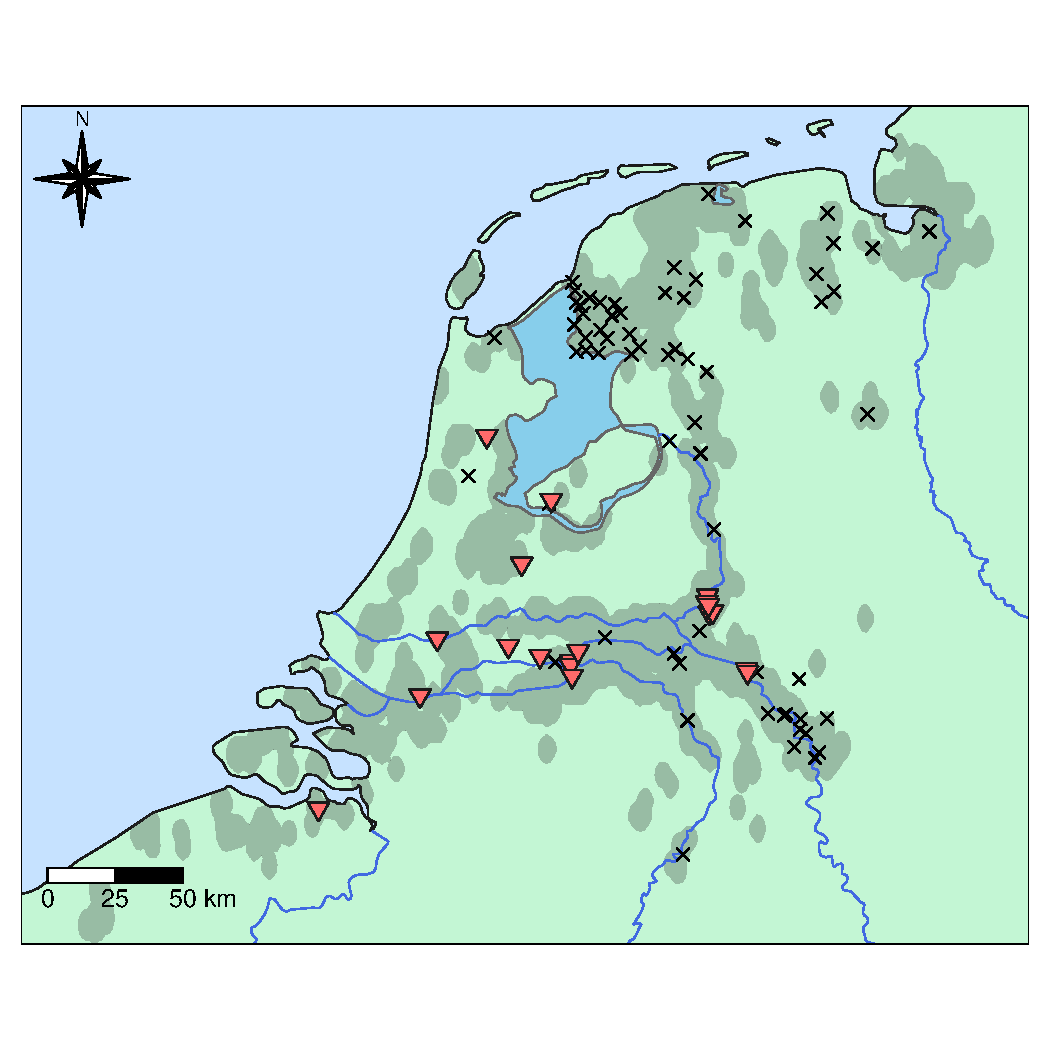
\includegraphics{datamap}

\caption{Using different datasets to map the development of family sizes in Greater White-fronted geese. Crosses represent sites from which flocks and families within were counted. Triangles show locations where GPS tracked goose families split. Grey polygons show a kernel around all sites at which a goose bearing a numbered neckband was observed. Lines represent rivers, lakes, and coasts.}

\end{figure}

\end{minipage}

\section{Another data map}
\end{document}
